\documentclass[12pt]{article}
\usepackage[T1]{fontenc}
\usepackage{geometry}
\geometry{verbose,tmargin=0.5in,bmargin=0.5in,lmargin=0.75in,rmargin=0.5in}
\pagestyle{headings}
\usepackage{color}
\usepackage{graphics}
\usepackage{graphicx}
\newcommand{\versionnumber}{1.0}
\makeatletter


\begin{document}

\title{Beamline Manual\\\normalsize Version \versionnumber}
\author{FX. Girod, K. Moffeit, T. Maruyama, S. Stepanyan}
\maketitle



\section{Contacts\label{beamline_contacts}}

\begin{description}
\item [Beamline~cell phone] (xxx) xxx-xxxx
\end{description}

The people listed in Table \ref{tab:calllist} should be called whenever there
is a problem beyond the on-hand expertise. The beam line expert is the main source for help.  
\begin{table}[tbhp]
\vspace{0.3cm}
{\centering \begin{tabular}{|c|c|c|c|}
\hline 
Who&Expertise&Cell Phone&Office\\
\hline 
\hline 
MCC&Beam tune, vacuum&&x7048 \& x7043\\
\hline 
Stepan Stepanyan&Beamline devices and applications&(757) 303-0499&x7196\\
\hline 
Francois-Xavie Girod&Beamline devices and applications&&x6002\\
\hline 
Engineering on call&General beamline&&\\
\hline 
\end{tabular}\par}
\vspace{0.3cm}


\caption{The beamline call list.\label{tab:calllist}}
\end{table} 



\section{What to Monitor along the Beamline}


\subsection{Beam conditions}

During data taking it is important to monitor the electron beam
to insure that changes in beam parameters do not effect data quality. For
example, changes in the beam halo can dramatically increase background rates
making the data worthless, or a change in the electron beam direction can cause
unwanted beam losses leading detector damage or beam trip. There are
automatic controls and alarms on beam conditions that will prevent beam damage to equipment 
and will terminate beam delivery in an event of beam excursion. Nevertheless,  the shift taker must
continuously monitor the beam parameters and act accordingly.

\subsubsection{Beam Current}

A consistent reading between the Faraday Cup (see Section \ref{sec:fcup}) current
and the "nA" BPMs is one way
to check that the electron beam is cleanly transported to the beam dump (Faraday Cup). (Note: in some experiments, when beam current exceeds allowed 
limit for Faraday cup, $\sim 50$ nA, beam stopper will be inserted in front of the Faraday cup. During high current runs, consistency in measured beam currents with "nA" and "stripline" BPMs must be monitored). In addition to the inconsistency of beam current readings, the halo counters (see Section \ref{sec:scaler_a}) should
show an increased activity if the beam is scraping the beam pipe upstream or downstream
of the target. Also higher then normal rates in the detectors would be indicative
of scraping immediately downstream of the target.
After the initial beam tuneup reference numbers for the scalers will be posted
in the log book and are to be used as reference. 

In the event that there appears to be unacceptable beam losses the following course of action is recommended:

\begin{enumerate}
\item Stop taking data, and make an E-log entry flagging any data runs that may be
contaminated.
\item Call MCC and explain to the operator what has been observed and explain why
the tune is unacceptable.
\item Work with the MCC operator to come up with a game plan to fix the problem.
\item Document the solution and start taking data again.
\end{enumerate}

\subsubsection{Beam Halo}

The presence of a beam halo is usually observed by an increase count rate in
the beam halo counters (see Section \ref{sec:scaler_a}). Typically
the upstream counters are very quiet and any count rate above $\sim 200$Hz (after initial gain adjustments for a well tuned beam) is indicative
of a problem. Note that an increase count rate in the upstream beam halo counters
can also indicate an obstruction in the beam pipe or just a bad beam tune. To
further investigate the source of a large count rate in the upstream beam halo
counters a harp scan (see the "electron beam profile scan" procedure in Section \ref{sec:harp}) should be performed. 

If the beam halo is unacceptable, take the following steps:

\begin{enumerate}
\item Stop taking data, make an E-log entry.
\item Call MCC and explain to the operator what has been observed and why this tune
is unacceptable.
\item Work with MCC to solve the problem.
\item Document the solution and start taking data again.
\end{enumerate}

\subsubsection{Beam Position}

The beam position before HPS is available from three "nA" cavities, 2C21, 2C24, and 2H01 and two stripline BPMs, 2H00 and 2H02. They measure the beam position as well as the current. From
these five measurements the beam angle can be determined. Drifts more the \( \pm 0.1 \)mm
should be brought to the attention of MCC. Feedback system is used to keep the beam position stable. It uses BPM information to drive horizontal and vertical correctors. Before data taking, shift worker must confirm that the feedback system is active. Note, that at beam currents below $50$ nA only "nA" cavities are reliable. 

\subsection{Beamline Vacuum}

The beamline vacuum is monitored from the vacuum screen available from the MCC on EPICS screens. The vacuum tends to be of order \( 10^{-6} \) torr upstream of the shield wall (upstream tunnel), and of order \( 10^{-5} \) torr
near the tagger and the throughout the downstream beam line. Vacuum is tightly monitored and interlocked to the beam delivery. 


\subsubsection{Catastrophic Loss of Vacuum}

There are two thin windows that are components of the HPS beamline, the Hall-B tagger vacuum chamber window
and the photon exit window at the downstream end of the last Frascati dipole vacuum chamber. If either of these two windows fail under vacuum
load there are fast valves interlocked to pressure gauges which will close
automatically. These valves will limit the loss of vacuum to the small region  of the Hall B beamline. Valves are interlocked to the beam Fast Shutdown System (FSD) and beam will be shutoff in an event of vacuum loss.

If any of the valves close due to poor vacuum: 

\begin{enumerate}
\item notify MCC immediately, turn off the beam (if it is not already OFF)
\item call the engineering on call 
\end{enumerate}

\subsection{Magnet Power Supplies}

The Hall-B beamline and HPS have magnets for beam transport, and momentum analysis. In Table \ref{magnets} list of the magnets, their power supplies
and point of control (POC) are shown. The items listed with B
as the point of control will be controlled by staff in the counting
house. The vertical and horizontal correctors, and the tagger magnet are controlled
by MCC, but the shift taker should monitor their settings. The tagger
magnet power supply is interlocked to the machine Fast Shutdown System (FSD). Interlocks are activated if run requires dumping the beam in the tagger beam dump, e,g during the initial beam tune. When the tagger
trips off the beam will be automatically shut off. This interlock must 
be masked out when electron beam is put through the hall for the experiment. The HPS chicane dipoles, Frascati-1, HPS-dipole, and Frascati-2, are controlled by the shift personal. Two "frascatis" share the same power supply, so called the Hall-B mini-torus power supply. The HPS-dipole uses the Hall-B pair spectrometer power supply. Both power supplies are interlocked with FSD system. Beam delivery will be terminated if any if these power supplies will trip.

\begin{table}[tbhp]
\vspace{0.3cm}
{\centering \begin{tabular}{|c|c|c|c|c|}
\hline 
magnet&
power supply&
POC&
Function&
Status\\
\hline 
\hline 
MB2C21V&
&
MCC&
vertical kick&
Active\\
\hline 
MB2C21H&
&
MCC&
horizontal kick&
Active\\
\hline 
m{\o}ller A&
Dyna-B&
B&
M{\o}ller polarimeter&
Not used\\
\hline 
m{\o}ller B&
Dyna-C&
B&
M{\o}ller polarimeter&
Not used\\
\hline 
MB2C22H&
&
MCC&
horizontal kick&
Active\\
\hline 
MB2C23V&
&
MCC&
vertical kick&
Active\\
\hline 
raster\_h1&
Danfysik&
B&
first horizontal target raster&
Not used\\
\hline 
raster\_v1&
Danfysik&
B&
first vertical target raster&
Not used\\
\hline 
tagger&
Danfysik&
MCC&
bend beam to tagger dump&
Active\\
\hline 
MBD2H00H&
&
MCC&
horizontal kick&
Active\\
\hline 
MBD2H00V&
&
MCC&
vertical kick&
Active\\
\hline 
MBD2H02H&
&
MCC&
horizontal kick&
Active\\
\hline 
MBD2H02V&
&
MCC&
vertical kick&
Active\\
\hline 
Frascati-1&
Dyna-A&
B&
bend beam by 30 mrad&
Active\\
\hline 
HPS-dipole&
Danfysik&
B&
spectrometer magnet&
Active\\
\hline 
Frascati-2&
Dyna-A&
B&
bend beam by 30 mrad&
Active\\
\hline 
\end{tabular}\par}
\vspace{0.3cm}


\caption{List of the magnets along the Hall B beamline and their functionality.\label{magnets}}
\end{table} 

If the tagger or the HPS chicane dipoles do trip off or is set incorrectly take the following action:

\begin{enumerate}
\item Call MCC immediately, tell them to shut off the beam.
\item Make an E-log entry.
\item Restore magnets (have MCC restore the tagger) to the proper setting.
\item Restore beam, verify that the beam is incident on the viewer (at the tagger dump if the tagger is energized or at the downstream tunnel if electron run is in progress)
\end{enumerate}

\subsection{Magnet and Power Supply Beacons}

Near every magnet in Hall B there are \textcolor{red}{red flashing beacons} that indicate status of the magnets. If beacon is
 flashing then the magnet \textbf{\textcolor{black}{is
powered}} or \textbf{\textcolor{black}{can be powered}} at
any time. If you need to work near or on a magnet and the red light is flashing
you must turn off the supply. The dangers of working
near a magnet are limited to those associated with stray magnetic fields. All
the high current bus work is enclosed in protective shields so there is no shock
hazard. Of course the supply needs to be shut off and lock and tagged before
any of the protective shield is removed.

After any work that required the power supply to be lock and tagged a through
sweep of the magnet area for magnetic debris is required before the lock and
tag can be removed.


\section{Hall B Epics Control Screens}


\subsection{EPICS GUI Launcher}

The \emph{"hps\_epics"} (see Fig.\ref{hps_epics}) is a \emph{medm} screen that serves as an icon manager of
\emph{medm} screens. From this screen, the bulk of the epics applications can
be started. It is recommended that when finished with a particular \emph{medm}
screen, that application be terminated (\textbf{not iconized}). If the screen
is needed in the future, just launch it again from the \emph{"hps\_epics"}. In this
manner searching through all the degenerate icons is eliminated. 

To start the \emph{"hps\_epics"}:

\begin{itemize}
\item log onto \textbf{clon01}

\item type: \textbf{hps\_epics}
\end{itemize}
\begin{figure}[htp]
{\centering 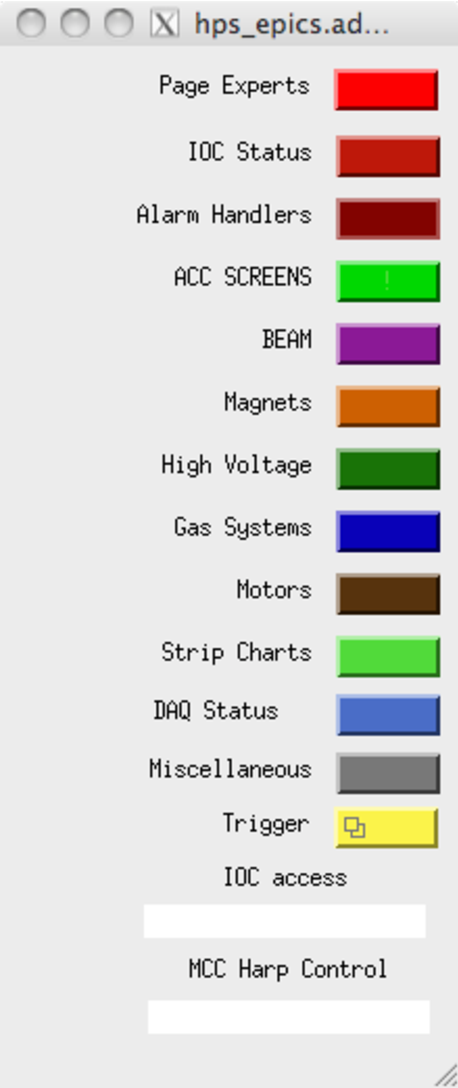
\includegraphics[scale=0.75]{hps_epics.pdf}\par}
\caption{\small{HPS EPICS GUI launcher.}}
\label{hps_epics}
\end{figure}


\subsection{Faraday Cup (classc4) \label{sec:fcup}}

The instantaneous beam current reading from the Faraday cup is available on
the \textbf{Main Scaler} screen as shown in Figure \ref{fig:scaler}. This GUI can be launched
via the \emph{"hps\_epics"} by selecting the \textbf{Beam}
pull down menu. The update rate is the same as for the beam halo scalers and
is controlled from that GUI, see Section \ref{sec:scaler_a}. An important consideration
is that the Faraday Cup current integrater rate is 10 counts/sec when the current
is 1 nA. This means that if the count time on the scaler is less than 1 sec
you will observe large statistical flucations.


\subsubsection{Beam blocker}

The Hall-B Faraday cup is not cooled and cannot operate at high currents (especially at high energies). If run requires use of beam currents above $50$ nA, beam blocker, cooled copper absorber, must be position in front of the Faraday cup. The beam blocker control GUI is shown in Figure \ref{beamblocker}.  Push "Go beam" button  in order to put the blocker on the beam and "Go Home" to retract if from the beamline. 

\begin{figure}[tbhp]
{\centering 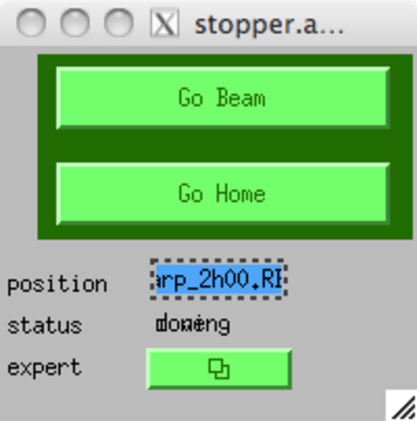
\includegraphics[scale=0.75]{beam_stopper.pdf} \par}
\caption{The beam blocker GUI. \label{beamblocker}}
\end{figure}

\subsection{nA BPM Displays}

The readout of na BPMs are displayed on the main scaler GUI as well as on BPM GUI, Fig. \ref{fig:bpm}. The BPM screen can be launched
via the \emph{"hps\_epics"} by selecting the \textbf{Beam}
pull down menu.
\begin{figure}[tbhp]
{\centering 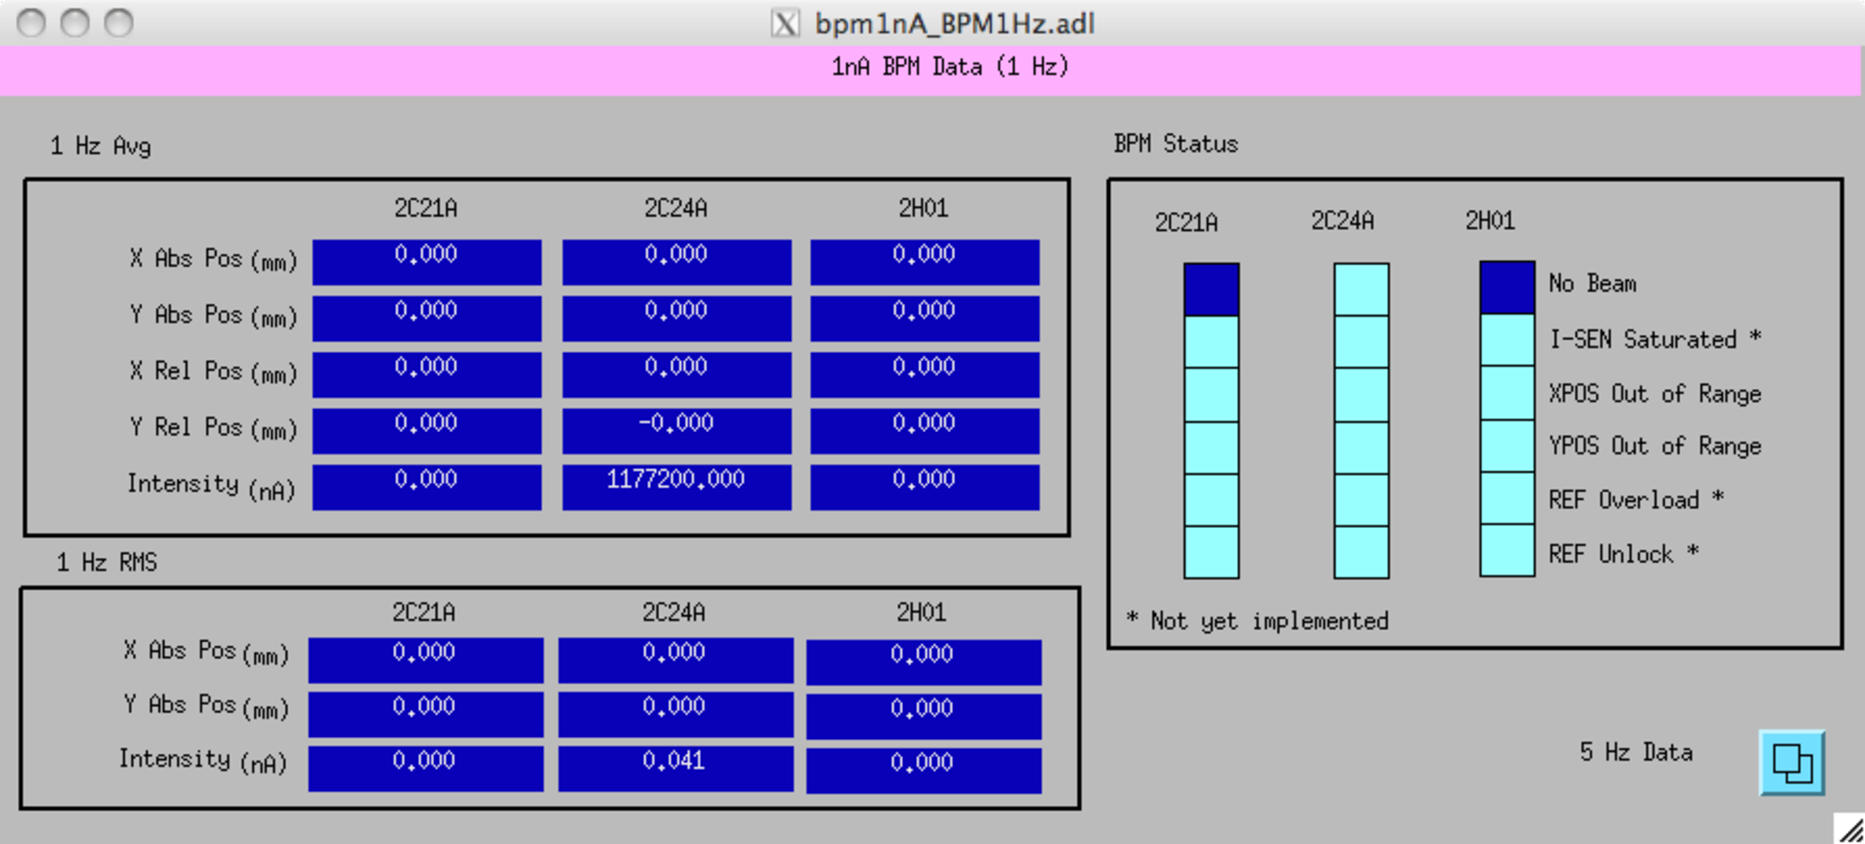
\includegraphics[scale=0.5]{bpms.pdf} \par}
\caption{The Hall B current screen. The current reading, in nAmps. The Faraday Cup current
reading is updated at the same rate as the beam halo scalers. \label{fig:bpm}}
\end{figure}

\subsection{Beam Halo Counters (classc1/classc4) \label{sec:scaler_a}}

The beam halo counters consist of photomultiplier tubes strapped to the beampipe along the beam line. There are two halo counters 
upstream of the Hall-B tagger magnet, two are installed on top of the tagger magnet vacuum box, four counters located in the apex of the forward carriage, two counters
downstream of the Frascati-1 and one counter downstream of the target, between HPS dipole and the Frascati-2. The beam halo counter scalers are displayed on the main scaler GUI. The GUI also
displays the Faraday Cup beam current, information from BPMs, rates in detectors (e.g. calorimeter), magnet settings, motor position (e.g. target). This display is launched via the Beam menu on the \emph{"hps\_epics"}.

\begin{figure}[tbhp]
{\centering \resizebox*{0.8\textwidth}{!}{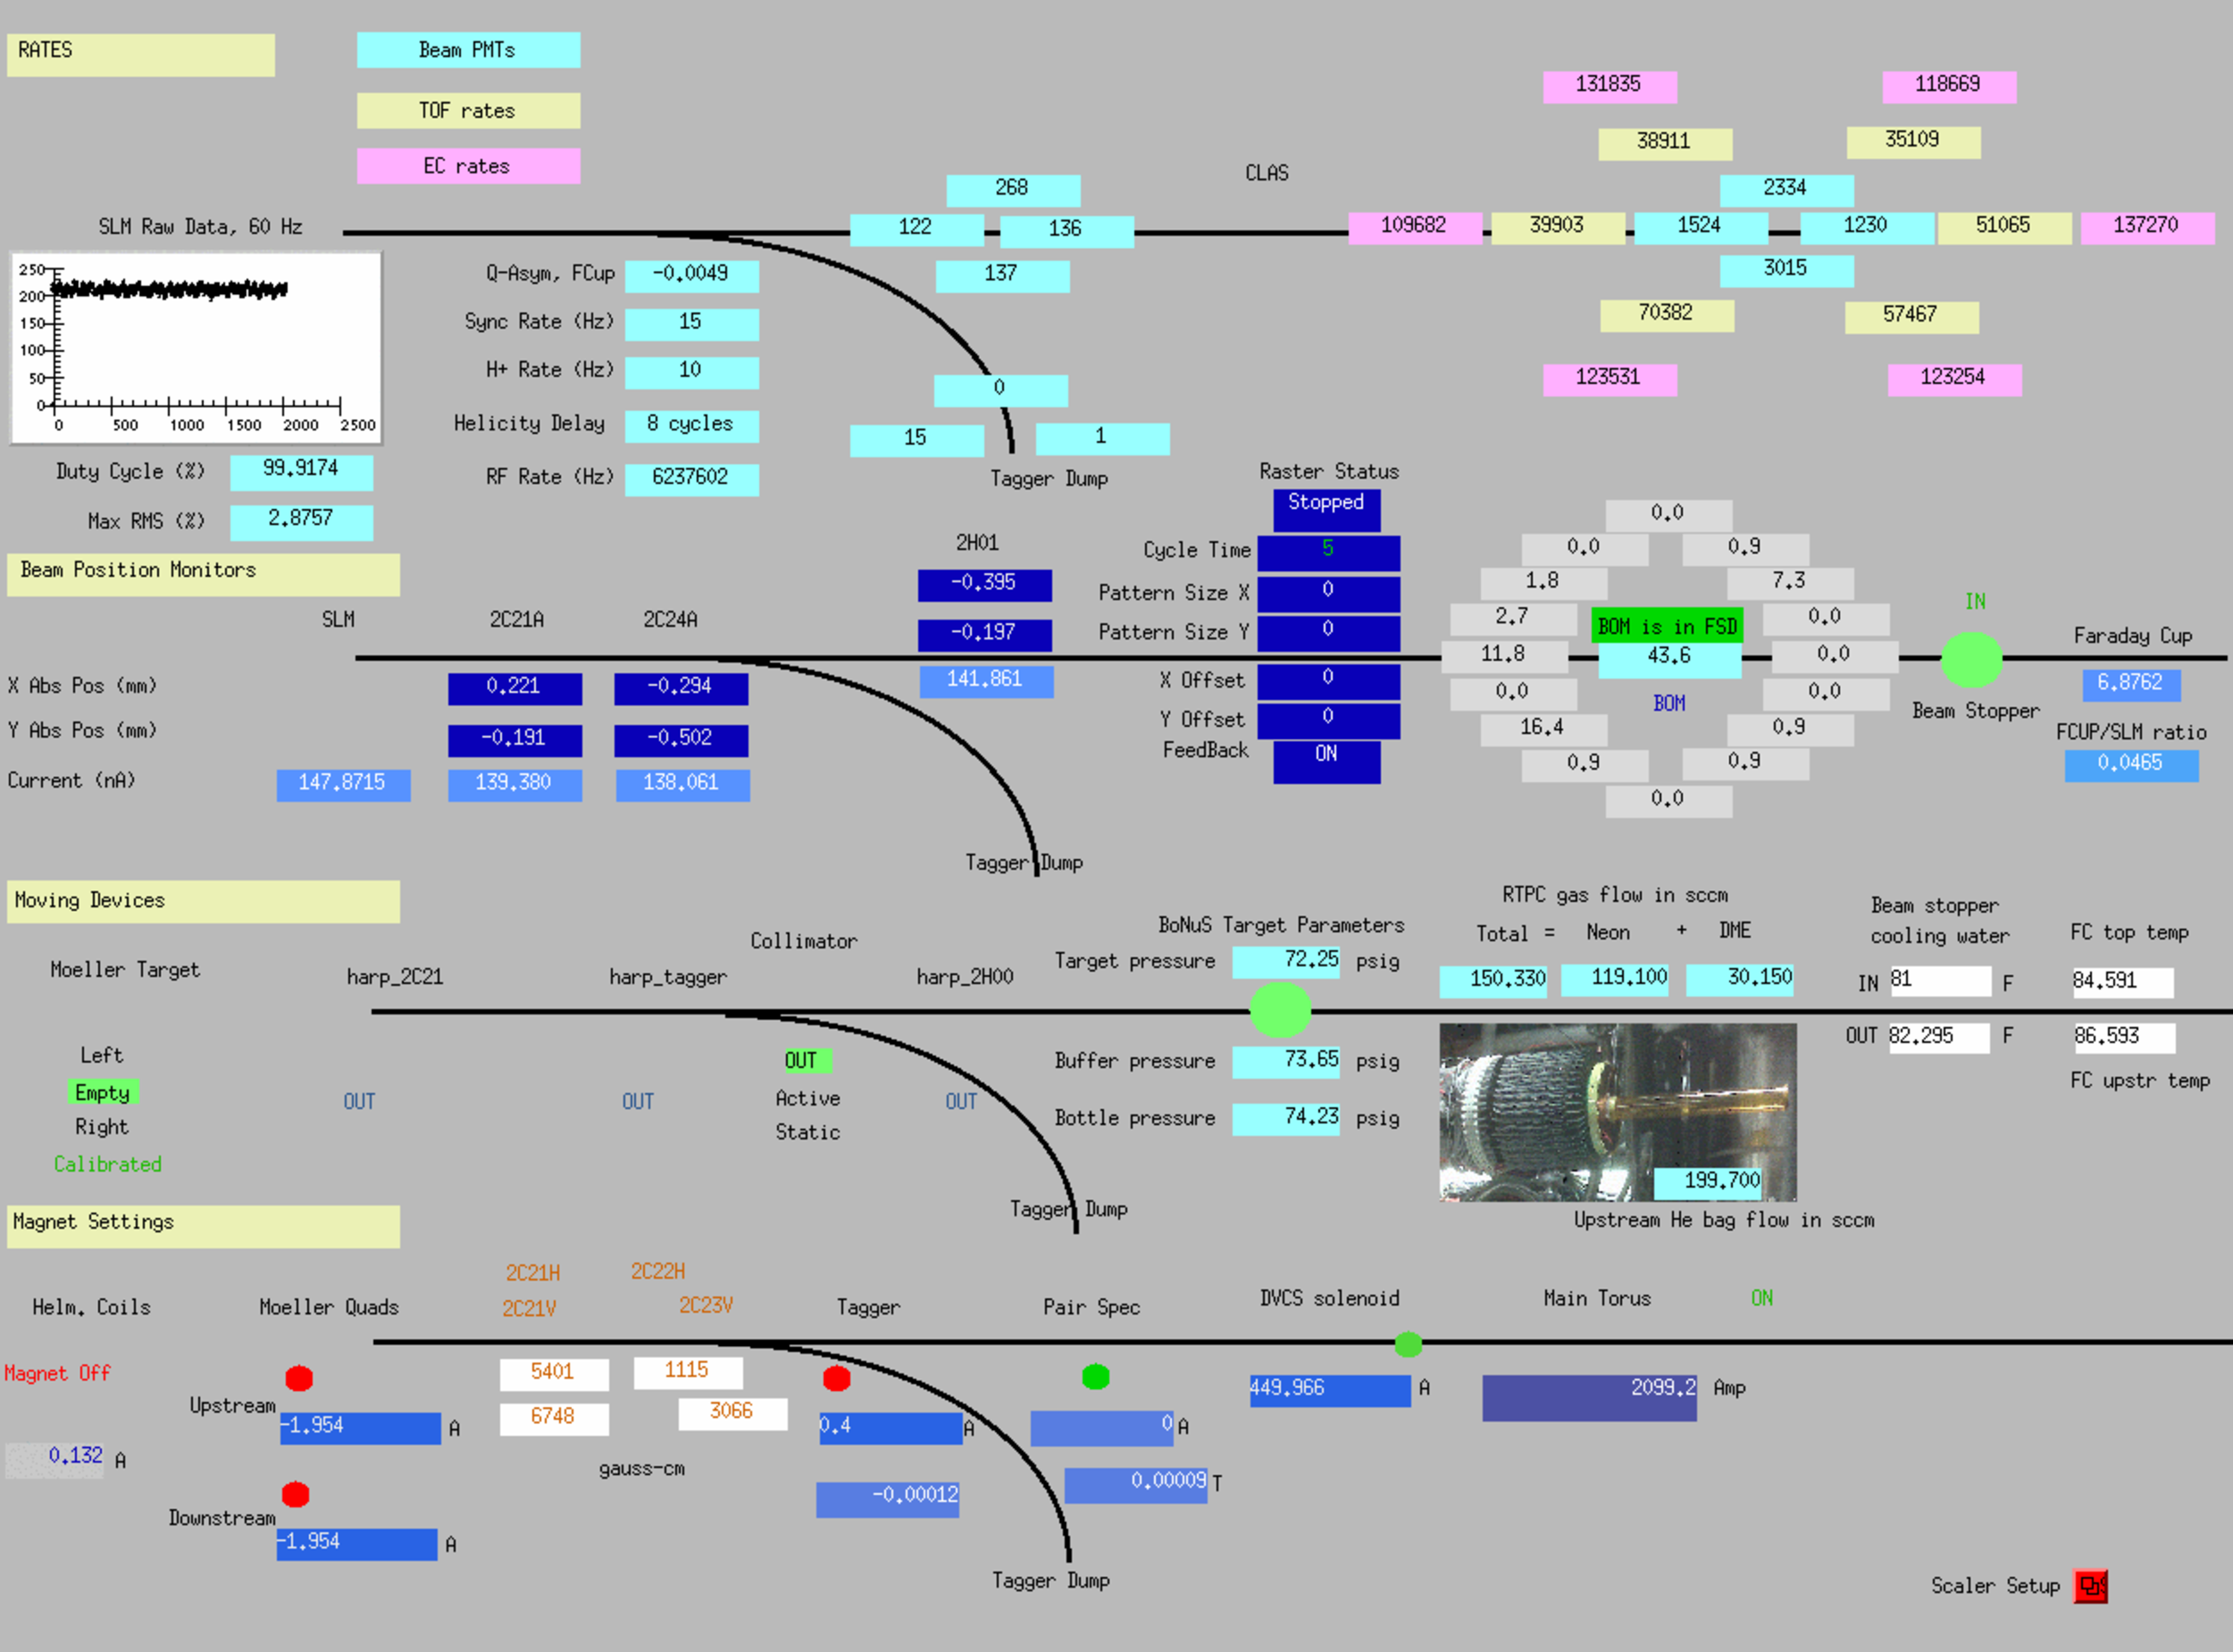
\includegraphics{scaler_4He.pdf}} \par}
\caption{The main scaler GUI.}
 \label{fig:scaler}
\end{figure}

\clearpage

\subsection{\bf Target}

Figure \ref{target} shows the HPS target. The 4$\mu$m-thick tungsten is used for 1.1 GeV and 2.2 GeV data taking, and the 8$\mu$m-thick tungsten is for 4.4 GeV and 6.6 GeV. The graphite and CH$_2$ targets are for calibration.

\begin{figure}[ht!]
\centering
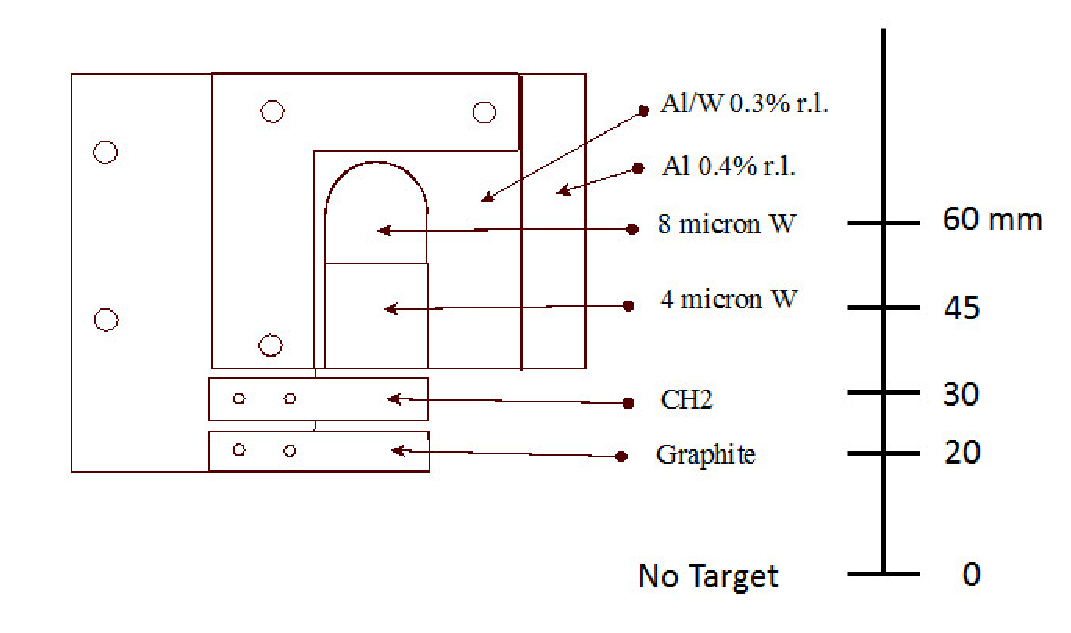
\includegraphics[width=15cm]{target.eps}
\caption{HPS target.}
\label{target}
\end{figure}

\subsubsection{\bf Setting the target}

Target can be set by running the target GUI (Figure \ref{targetgui}).

\begin{itemize}
\item
Type in who you are.
\item
Call MCC to turn off the beam and click ``Have you called MCC to turn off the beam?''.
\item
Hit appropriate target button.
\item 
Hit ``Remove Target'' button to remove the target.
\end{itemize}

Your name and Date and Time will be logged. The target will be placed at the nominal beam position. By providing an offset value, the target position can be adjusted vertically.

\begin{figure}[ht!]
\centering
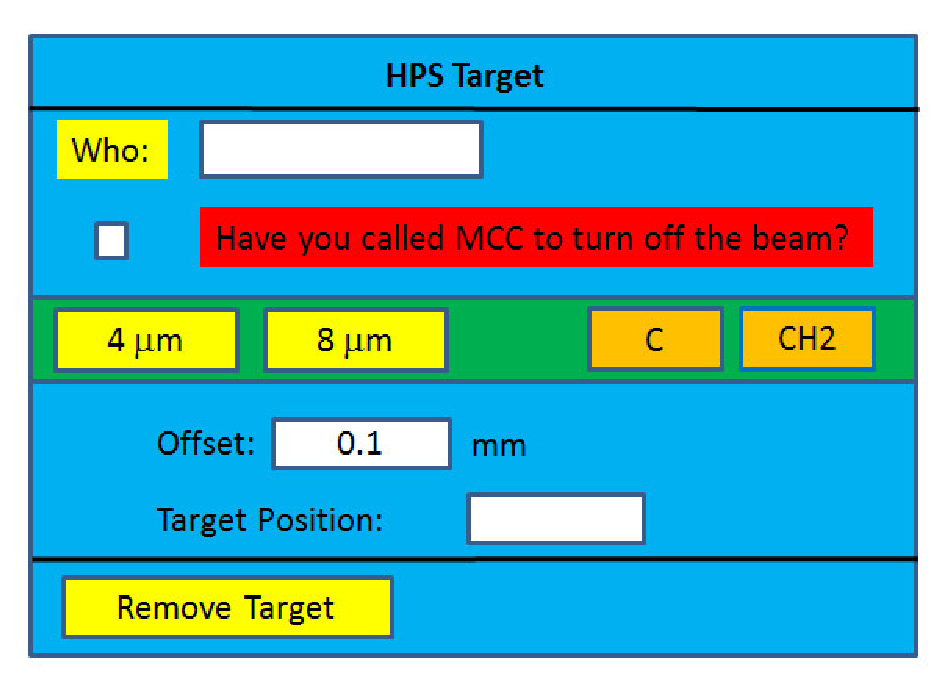
\includegraphics[width=10cm]{targetgui.eps}
\caption{Target GUI}
\label{targetgui}
\end{figure}


\subsection{Hall-B Harps (classc3)\label{sec:harp}}

There are three wire harps on the Hall B beamline, 2C21, "tagger" or 2C24, and 2H03 (will be renamed to 2H00 for CLAS running). The harp launch GUI, Figure \ref{harpmain}, enables operator to open control GUI for the desired harp. A stepper motor in conjunction
with the beam halo scalers is used to perform a beam profile measurements. The harp operation is controlled from the Harp GUI, see Figure \ref{taggerharp}. During a scan the beam
halo scaler GUI is controlled by the scan application (see Section \ref{sec:scaler_a}).

\begin{figure}[tbhp]
{\centering \resizebox*{0.4\textwidth}{!}{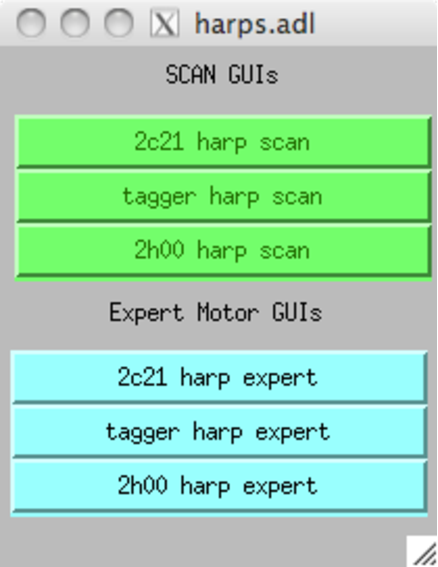
\includegraphics{harps.pdf}} \par}
\caption{The main Harp medm screen. The green buttons on the top are for opening individual harp control. Cyan buttons below for expert GUIs.}
\label{harpmain}
\end{figure}

In order to perform a harp scan one should push "SCAN" button. After the scan finished (motor position has been restored at $0.0$ position) use "Analyze Scan Data" to see beam profile and fit results to the scaler distributions.
\begin{figure}[tbhp]
{\centering \resizebox*{0.75\textwidth}{!}{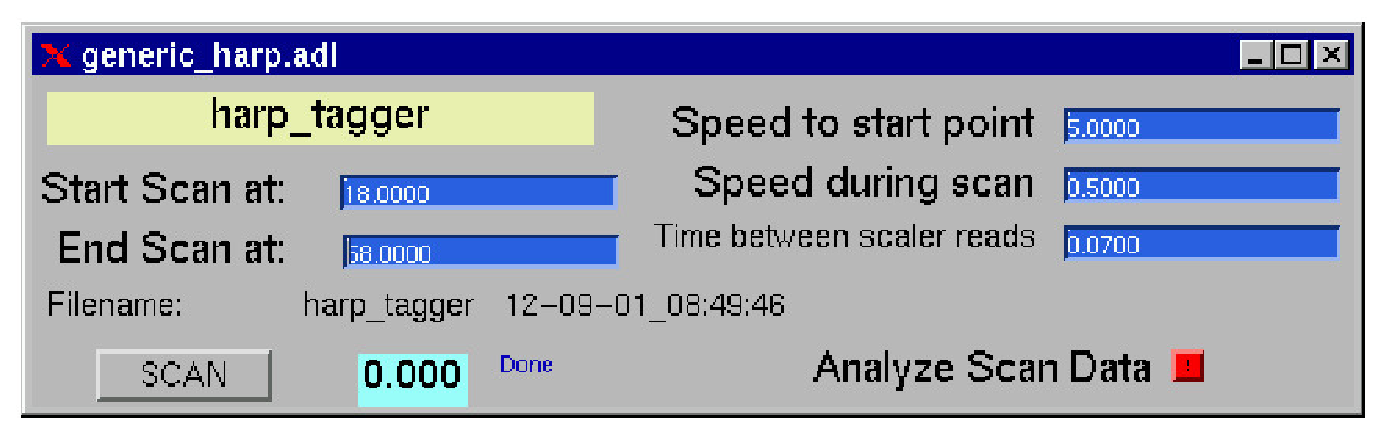
\includegraphics{harp.eps}} \par}
\caption{The tagger harp medm screen. This GUI controls a stepper motor and the halo counter scaler settings.}
\label{taggerharp}
\end{figure}

\clearpage
\subsection{SVT Protection Collimator\label{collimators}}

Figure \ref{collimator} shows the SVT protection collimator. ``3 mm gap'' and ``2 mm gap'' are 1cm-thick Tungsten collimator with a 3 mm gap and 2 mm gap, respectively. ``3 mm gap + Foil'' has a 10$^{-4}$ r.l. Gold foil at the downstream surface. The nominal positions in the collimator coordinate are,

\begin{itemize}
\item
Collimator out:  0 mm
\item
Wire: 20 mm
\item
Middle of 3 mm gap : 50 mm
\item
Middle of 3 mm gap + $10^{-4}$ r.l. Gold Foil: 80 mm
\item
Middle of 2 mm gap: 110 mm
\item
$10^{-4}$ r.l. Gold Foil: 140 mm
\end{itemize}

\begin{figure}[ht!]
\centering
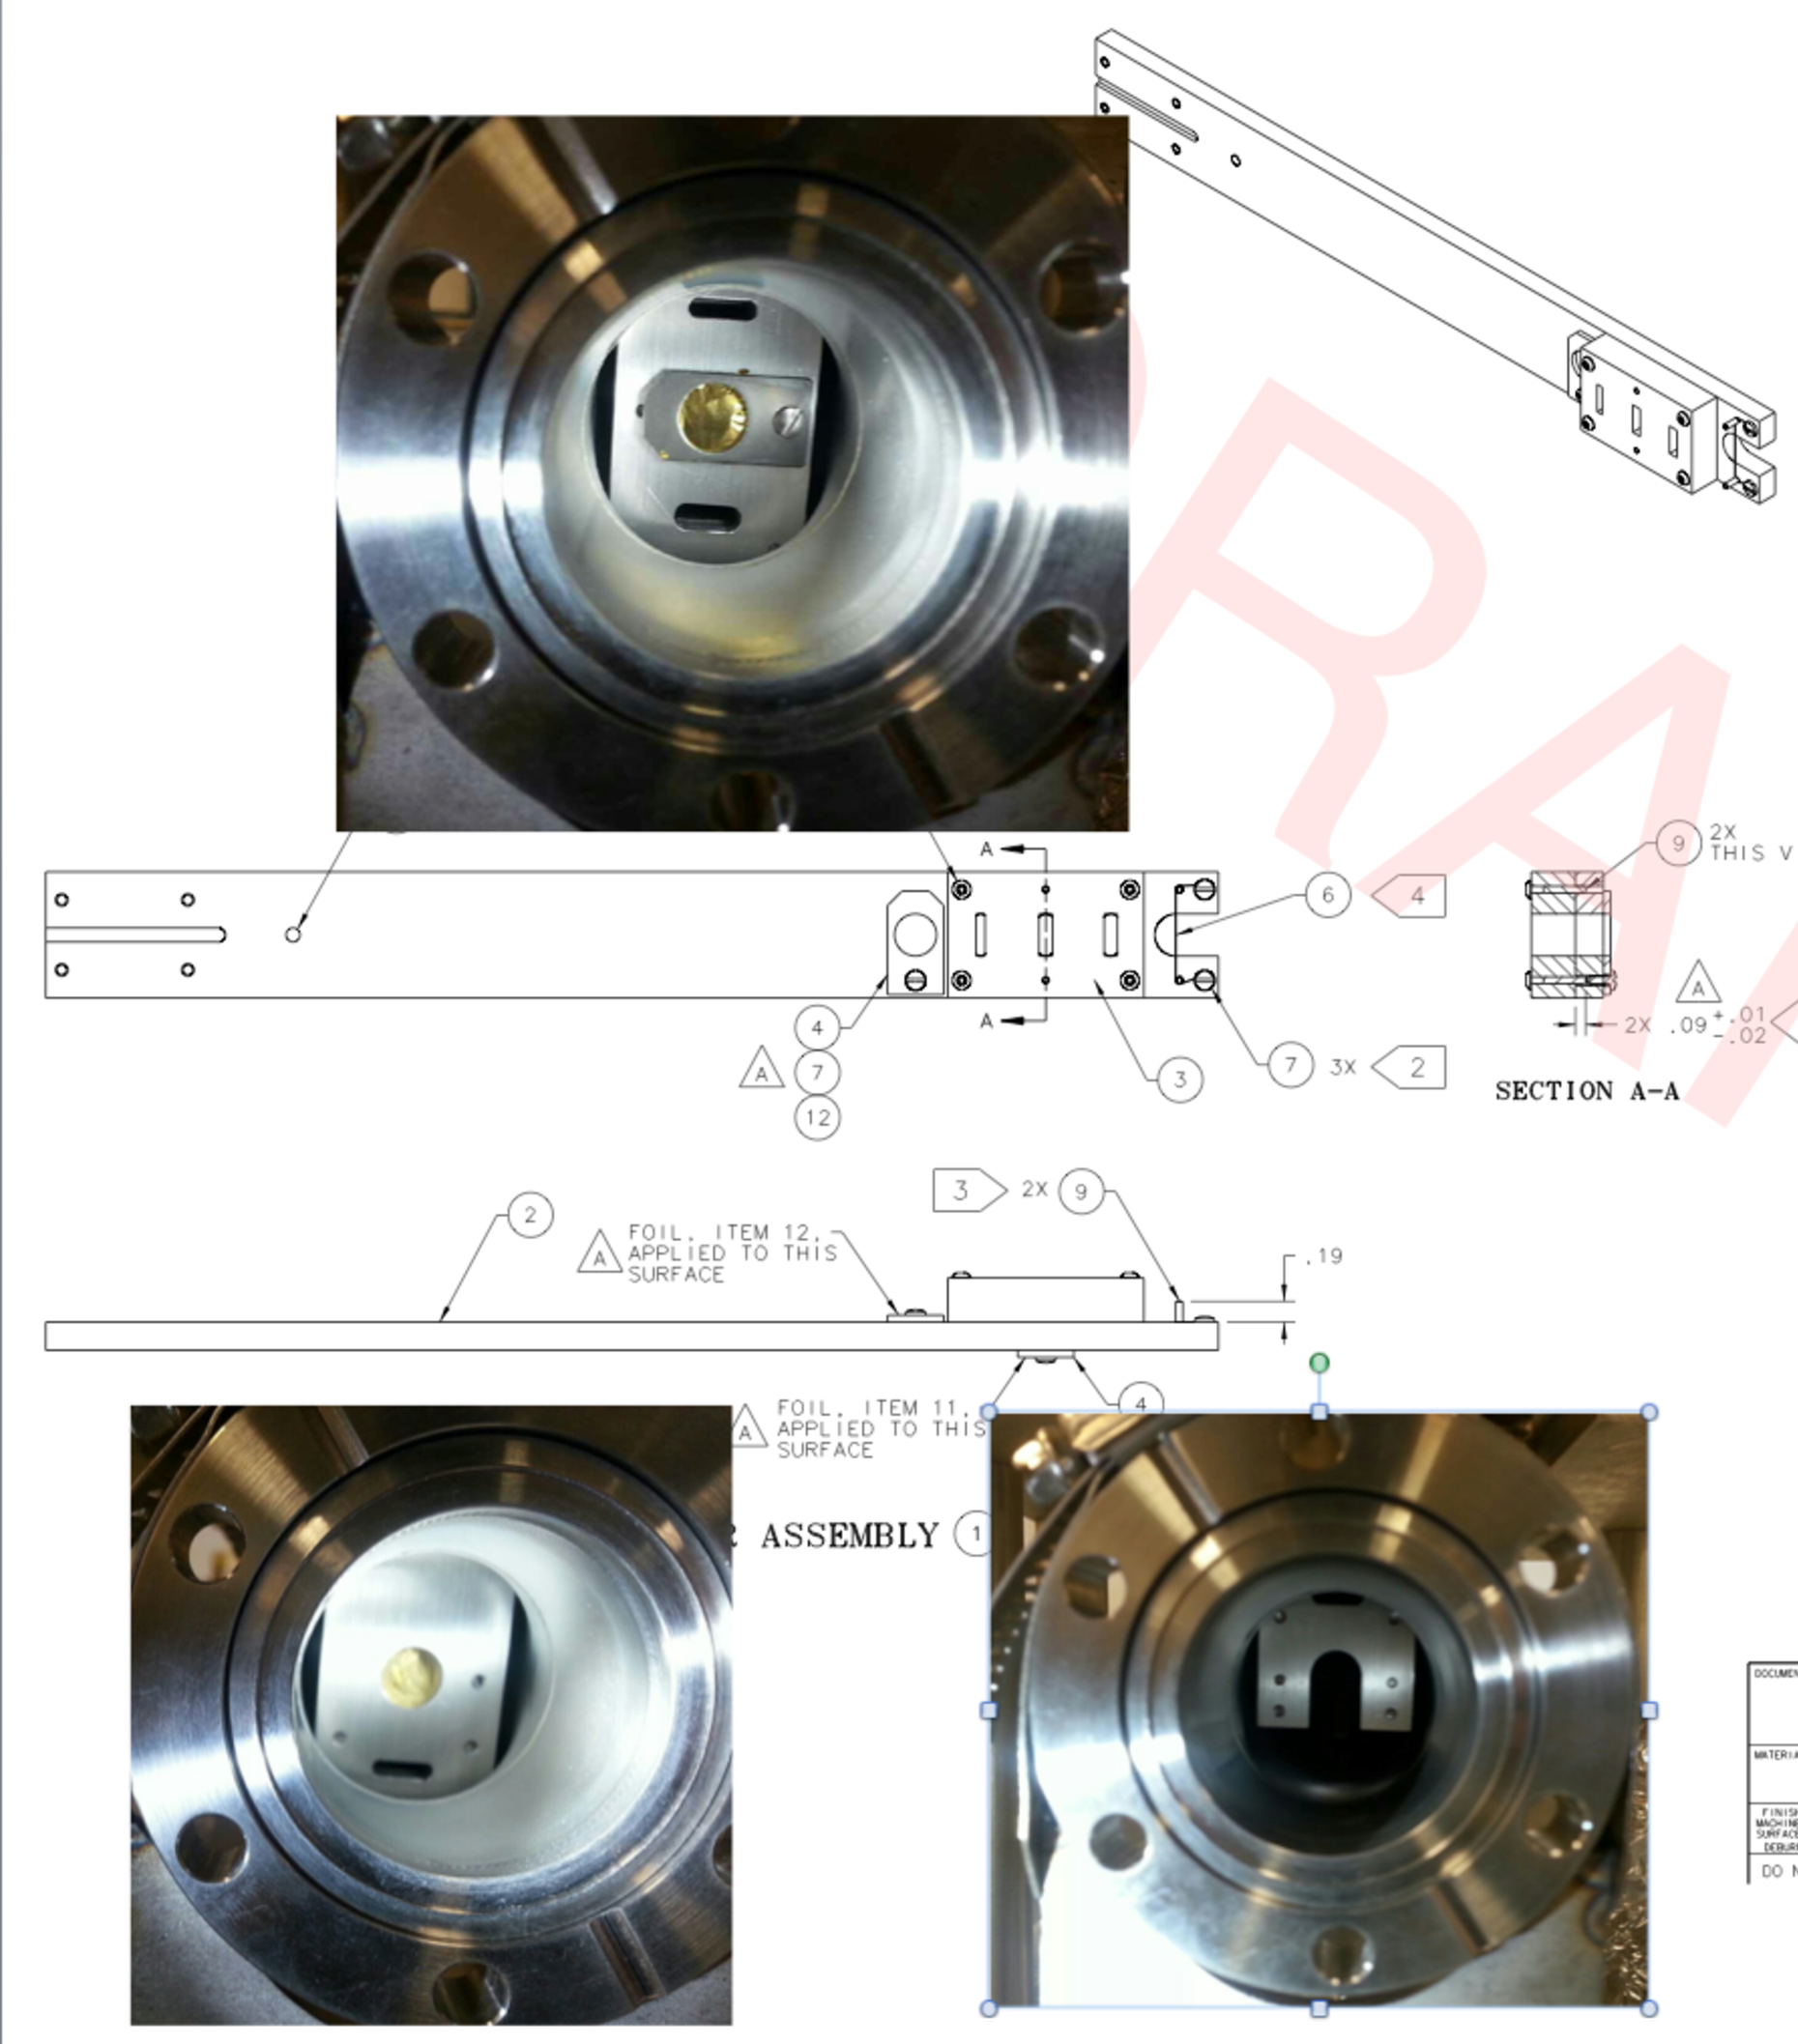
\includegraphics[width=15cm]{svt_collimator.pdf}
\caption{SVT Protection Collimator}
\label{collimator}
\end{figure}

\subsubsection{\bf Wire Scan}

\noindent
{\bf Setup}

\begin{itemize}
\item
MCC is not moving the beam or changing beam conditions
\item
Ask MCC to mask Halo Counters in FSD as we are doing Collimator Wire Scan.
\item
SVT is fully retracted and the power is off.
\item
ECal is operational.
\item
Downstream Halo Counter is operational.
\end{itemize}

\noindent
{\bf Scan}

A wire scan can be performed from the wire scan GUI (Figure \ref{taggerharp}) which is launchable from {\it clas epics}. Once the scan is completed, the collimator will move to ``out'' position.

\begin{itemize}
%\item Type in who you are.
\item
Click ``scan'' using default values.
\item
When the motor is ``Done'', click the red button to the right of ``Analyze Scan Data''.
\item
Choose either ECal or Halo Counter as the detector. 
\item
Find the beam offset ($\Delta$y) from the nominal beam position (y=20 mm).
\end{itemize}

\begin{figure}[ht!]
\centering
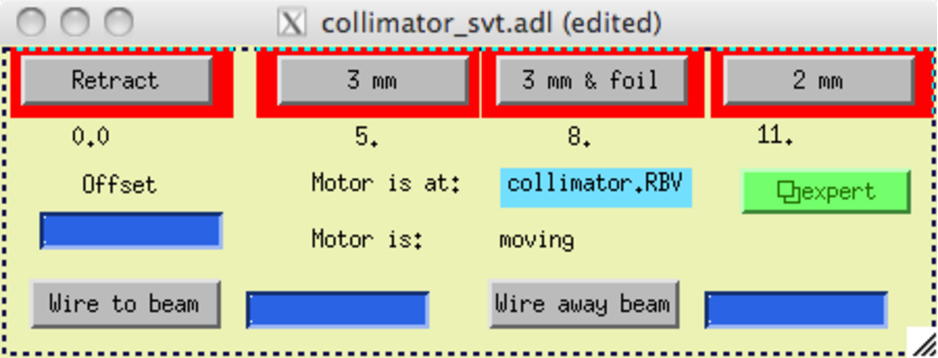
\includegraphics[width=12cm]{svt_collimator_GUI.pdf}
\caption{SVT protection collimator control GUI.}
\label{svtcollimator}
\end{figure}

\subsubsection{Setting the collimator}

Once the beam offset is measured, the collimator can be set by running the collimator GUI shown in Figure \ref{svtcollimator}.

\begin{itemize}
%\item Type in who you are.
\item Call MCC to turn off the beam 
%and click ``Have you called MCC to turn off the beam?''.
\item Type in the beam offset value.
\item Hit ``3 mm + Foil'', ``3 mm gap'', or ``2 mm gap'' button.
%\item  Hit ``PANIC'' button to abort.
\end{itemize}

%\begin{figure}[ht!]
%\centering
%\includegraphics[width=12cm]{CollimatorGUI.eps}
%\caption{Collimator GUI}
%\label{collimator}
%\end{figure}

If you don't provide the beam offset, the collimator will be set at the nominal position. If you provide the beam offset and hit ``Reset'', the collimator nominal position will be reset by this value. The collimator position can be fine tuned by providing an arbitrary offset value. However, maximum offset value is limited to 1 mm for the 3-mm gap and 0.5 mm for the 2-mm gap.

Hitting ``Rettract' moves the collimator to y=0 mm.
 

\subsection{Magnets}


\subsubsection{Mini-Torus Magnet(classc3)\label{sec:minit}}

The "Frascati-1 and Frascati-2 dipoles are controlled by the Hall-B mini-torus magnet GUI (see Figure \ref{fig:minit}) launchable
from "Magnets" of the \emph{"hps\_epics"}. The magnet current settings vary depending on the run
conditions, check with the shift leader, Run Coordinator or PDL if you are unsure
of the appropriate current setting. The power supply is $10000$ A/$30$ V supply. In EPICS control system of this power supply the max current to the magnets will be limited to $1200$ A. 

\begin{figure}[tbhp]
\resizebox*{0.9\textwidth}{!}{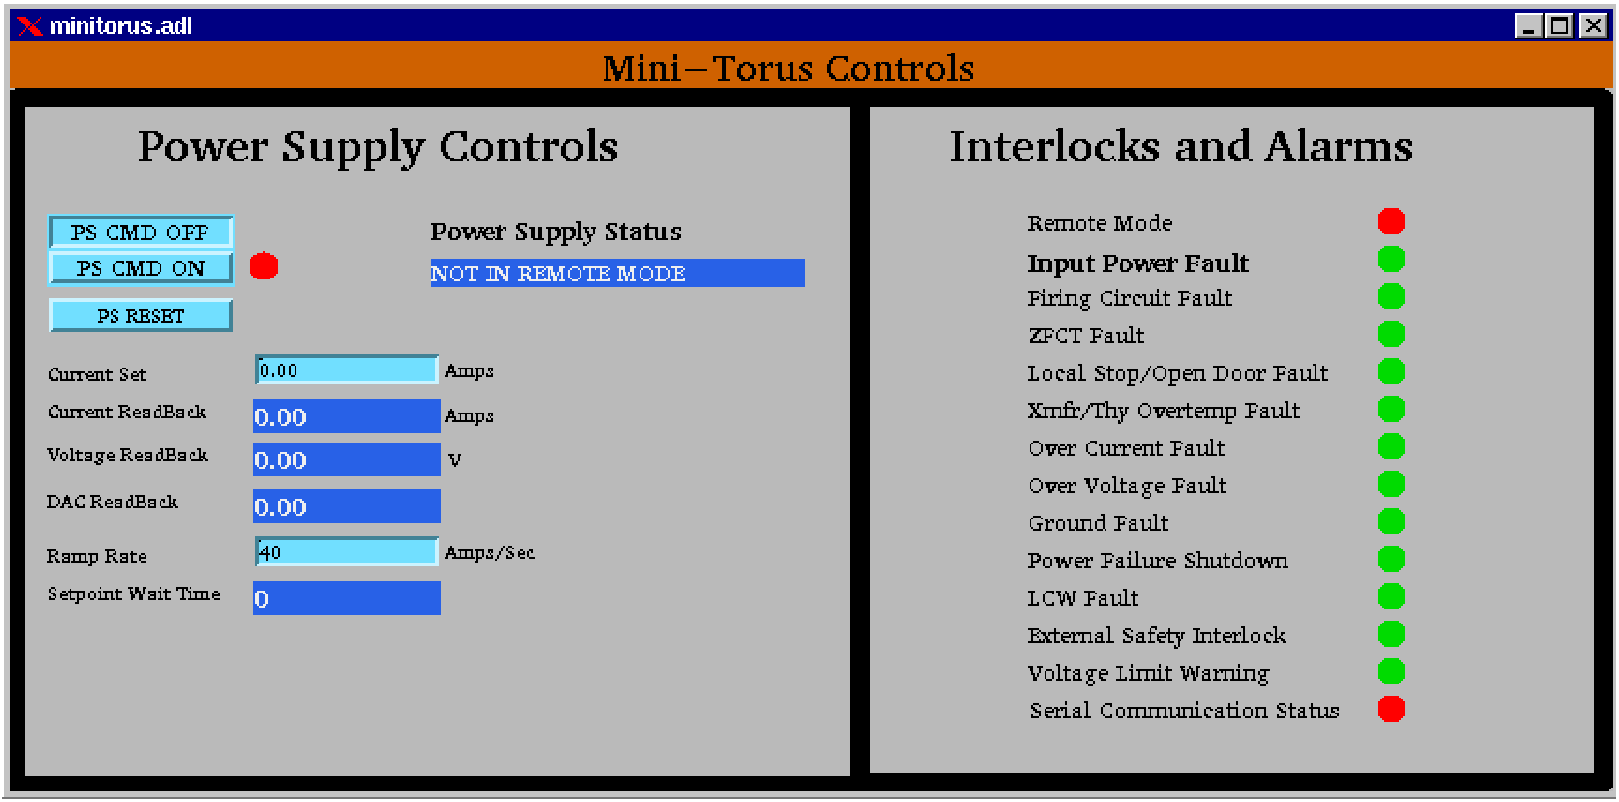
\includegraphics{minitorus.pdf}} 
\caption{The mini torus power supply control GUI. \label{fig:minit}}
\end{figure}


\subsubsection{HPS-dipole Magnet(classc3)\label{pair_spectrometer}}

The HPS-dipole magnet is fed from the Hall-B pair spectrometer magnet power supply. The power supply is controlled by a GUI (see Figure \ref{pairspecgui})
launchable from "Magnet" of the \emph{"hps\_epics"}. The magnet current
settings vary depending on the primary electron beam energy,
check with the shift leader, Run Coordinator or PDL if you are unsure of the
appropriate current setting. The magnet and power supply can operate up to \~{}3600Amps.

\begin{figure}[tbhp]
\resizebox*{0.9\textwidth}{!}{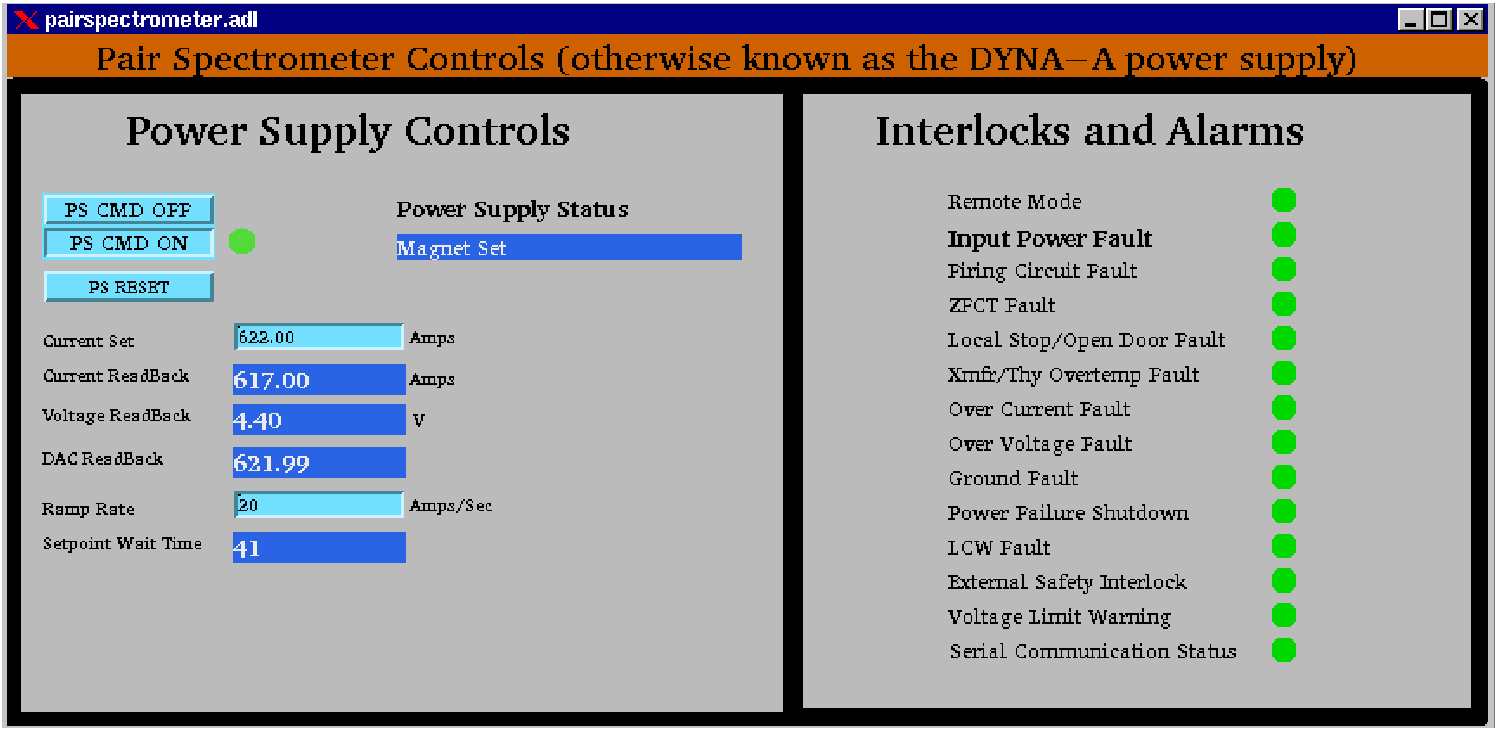
\includegraphics{pair_spectrometer.pdf}} 
\caption{The mini torus power supply control GUI. \label{pairspecgui}}
\end{figure}




\end{document}
